\chapter{Modelling language competition on a complex network}

\section{Model presentation}

Our global language heritage is at risk: about 50\% of the 6,000 languages spoken today may face extinction this century. In this context, simple models describing language competition can offer useful insights for policy-making.

A dynamical analysis of different networks can clarify the interplay between language competition and social aggregation. Our analysis strems from the Abrams and Strogatz model, which explores endangered language dynamics \cite{Ambrams2003}. Their study considers a two-state society, with speakers of \textbf{language A} or \textbf{language B}, and describes the system's evolution using an ODE to derive transition probabilities.

\begin{comment}
$P_{yx}(x,s)$:
\begin{equation}
\label{Strogatz}
 \frac{dx}{dt}=yP_{yx}(x,s)-xP_{yx}(1-x,1-s)
\end{equation}
where \textit{x} is the fraction of \textbf{A}'s speakers, $\textit{y=1-x}$  is the fraction of \textbf{B}'s speakers and $0\leq \textit{s}\leq 1$ is a measure of \textbf{A}'s relative status.
\end{comment}

The model predicts that one language will eventually drive the other to extinction. However, since bilingual societies exist, the model requires refinement to account for this behavior.

Castelló et al. \cite{Castello2008} examine agents on three types of networks: regular, small-world, and social \cite{Toivonen2006}. They also introduce a bilingual state, \textbf{AB} (i.e., simultaneous use of both \textbf{A} and \textbf{B}) \footnote{We always refer to language use rather than competence. Thus, a person can leave the bilingual state at any time.}.

In this setup, agent \( j \) sits on a network, of \( N \) individuals, with \( k_j \) neighbors. The state of an agent evolves as follows: at each iteration, we choose agent \( i \) at random and compute the local densities of language users in the neighborhood of agent \( i \), denoted \( \sigma_i^l \) (where \( l \in \left\{ \textbf{A},\textbf{B},\textbf{AB}\right\} \text{ and } \sigma_i^A+\sigma_i^B+\sigma_i^{AB}=1 \)). Agent \( i \) changes state according to the following transition probabilities: \footnote{\textbf{A} and \textbf{B} have equal status: in fact eq (\ref{AB_eq}) are symmetric under the exchange of A and B.} \footnote{Note that transitions between monolingual \textbf{A} and monolingual \textbf{B} always pass through the bilingual state.}.


\begin{align}
\begin{array}{cc}
p_{i,A \to AB} = \frac{1}{2} \sigma_{i}^B & p_{i,B \to AB} = \frac{1}{2} \sigma_{i}^A \\[10pt]
p_{i,AB \to B} = \frac{1}{2} (1 - \sigma_{i}^A) & p_{i,AB \to A} = \frac{1}{2} (1 - \sigma_{i}^B)
\label{AB_eq}
\end{array}
\end{align}

Finally, for each network, results are compared to an agent-based version of the Strogatz two-state model:

\begin{align}
\begin{array}{cc}
p_{i,A \to B} = \frac{1}{2} \sigma_{i}^B & p_{i,B \to A} = \frac{1}{2} \sigma_{i}^A
\label{Strogatz_eq}
\end{array}
\end{align}

Our goal is to reproduce the results of Castelló et al. \cite{Castello2008} for lattice and small-world networks.



\section{Two-dimensional regular network}
In this lattice, each node has four neighbors under periodic boundary conditions (PBC). Each node \(i\) is assigned a vector component \(S_i\), which can take one of three possible values, representing different states. The initial configuration is randomly drawn from a uniform distribution.

We primarily use \textsl{igraph} for network manipulation and \textsl{ggplot2} for plotting. To speed up computations, nodes fully embedded in a uniform domain (not at the boundary) are excluded from the evolution algorithm.

As observed by Castelló, domains of monolingual communities undergo coarsening, with larger domains growing at the expense of smaller ones, while bilingual agents form narrow bands between monolingual regions. The system eventually reaches a dominance-extinction state.

Similar behavior is found in the agent-based Abrams-Strogatz model. However coarsening here is slower and driven by interfacial noise.
%before driven by surface dynamics...
Below are two snapshots of the dynamics: red nodes are in state A, black in state B, and white in AB.

\begin{figure}[h]
\centering
\begin{minipage}[t]{0.43\linewidth}
    \centering
    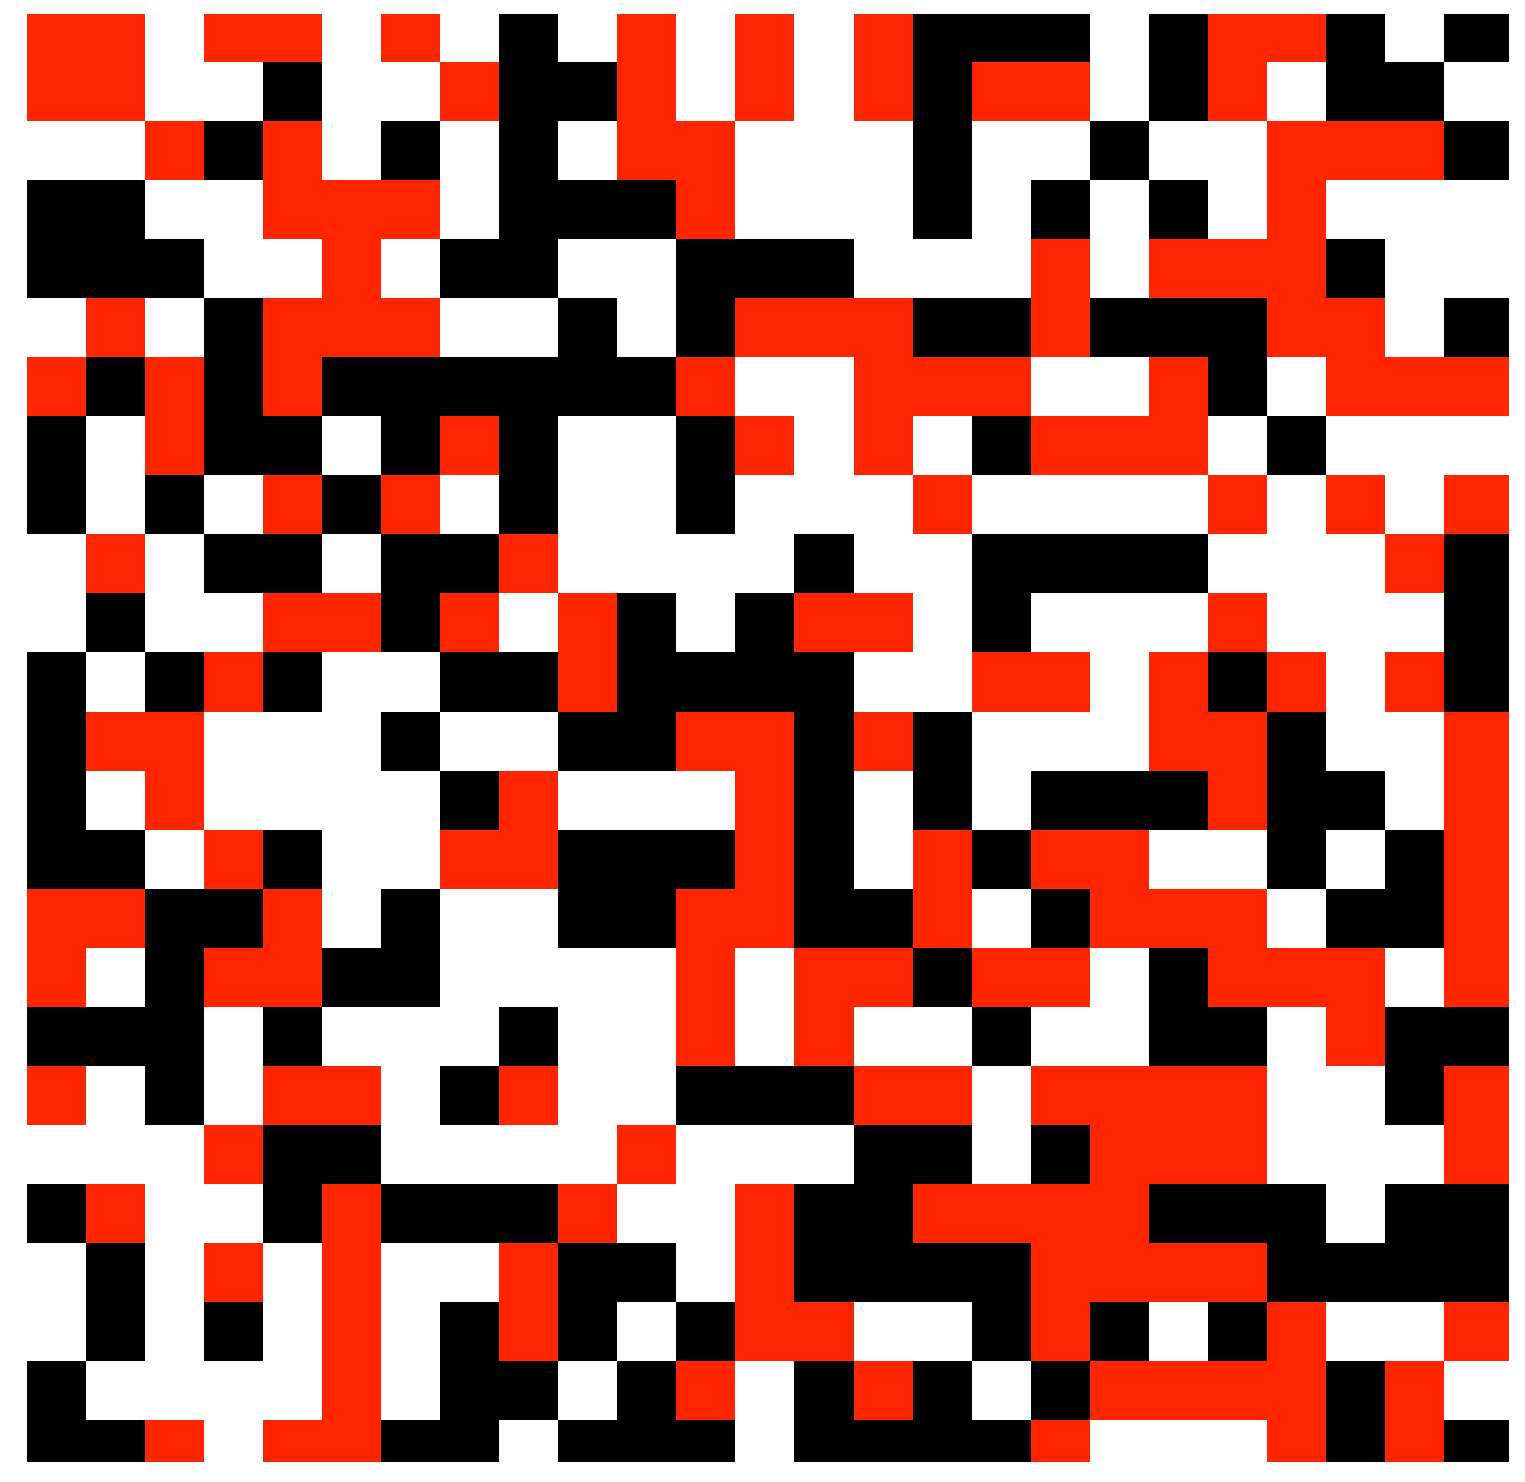
\includegraphics[width=\textwidth]{images/task1/regular_net_bi_t=1.png} 
    \caption{\scriptsize Bilingual, \(N=625\), \(t=0\)}
    \label{reg_net_bi1}
\end{minipage}
\hfill
\begin{minipage}[t]{0.43\linewidth}
    \centering
    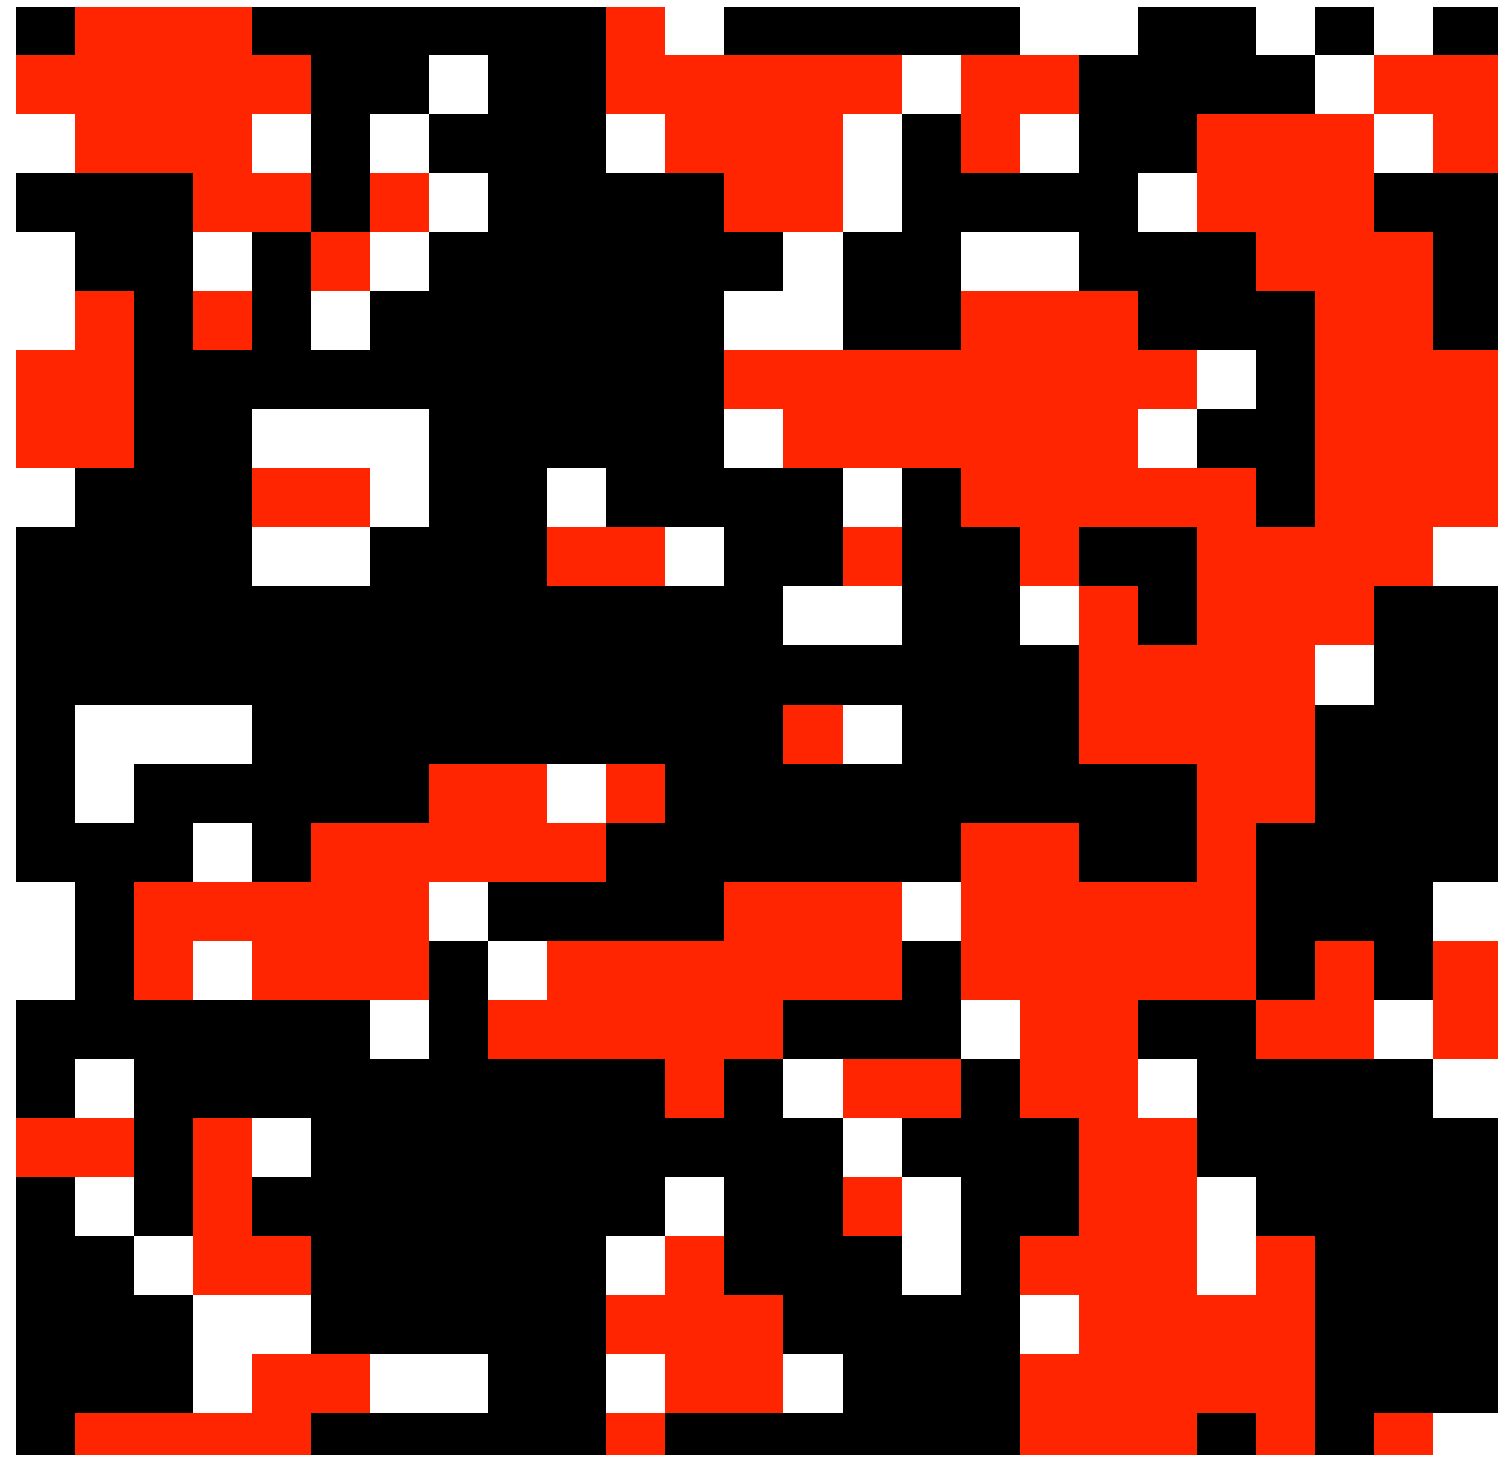
\includegraphics[width=\textwidth]{images/task1/regular_net_bi_t=5000.png} 
    \caption{\scriptsize Bilingual, \(t=5000\)}
    \label{reg_net_bi2}
\end{minipage}
\vspace{-5pt}
\begin{minipage}[t]{0.43\linewidth}
    \centering
    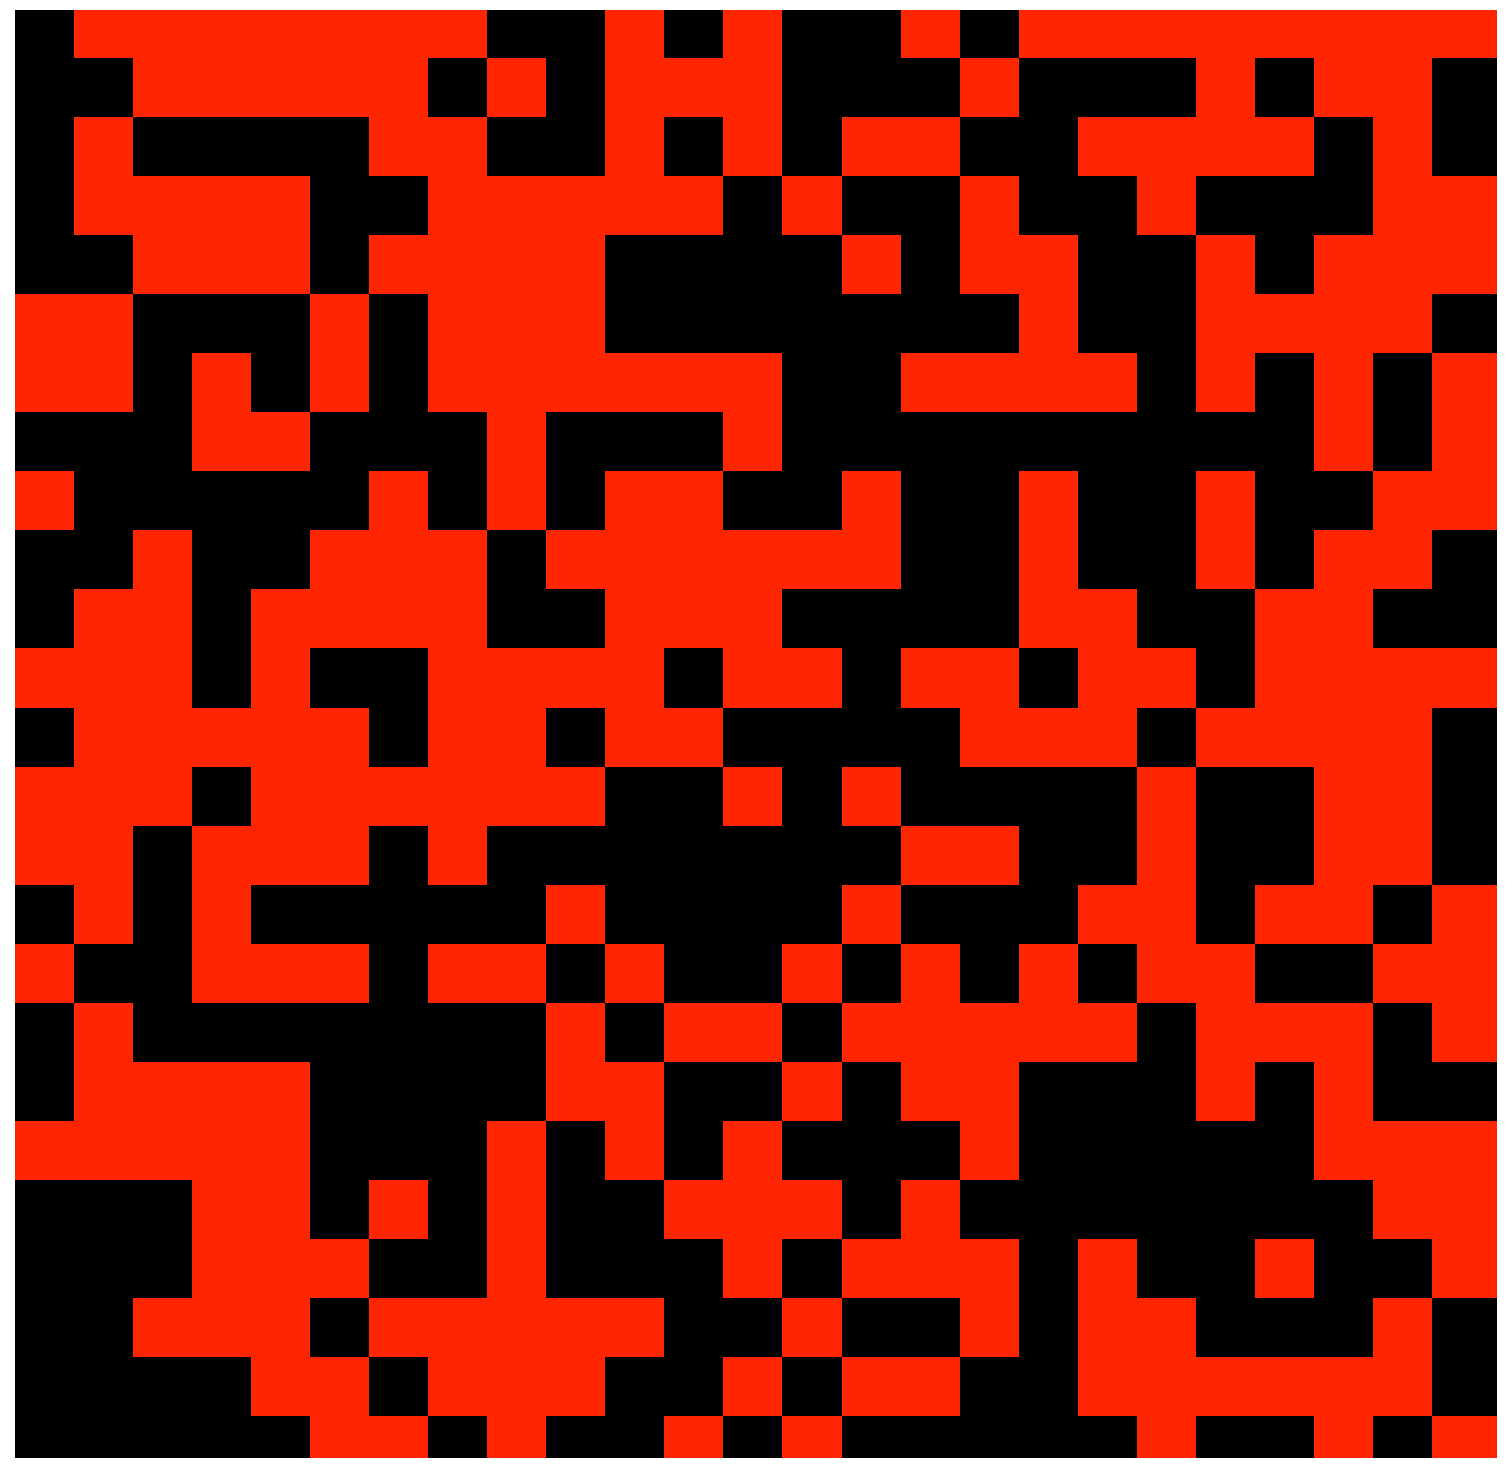
\includegraphics[width=\textwidth]{images/task1/regular_net_Str_t=1.png} 
    \caption{\scriptsize A-S model, \(N=625\), \(t=0\)}
    \label{reg_net_Str1}
\end{minipage}
\hfill
\begin{minipage}[t]{0.43\linewidth}
    \centering
    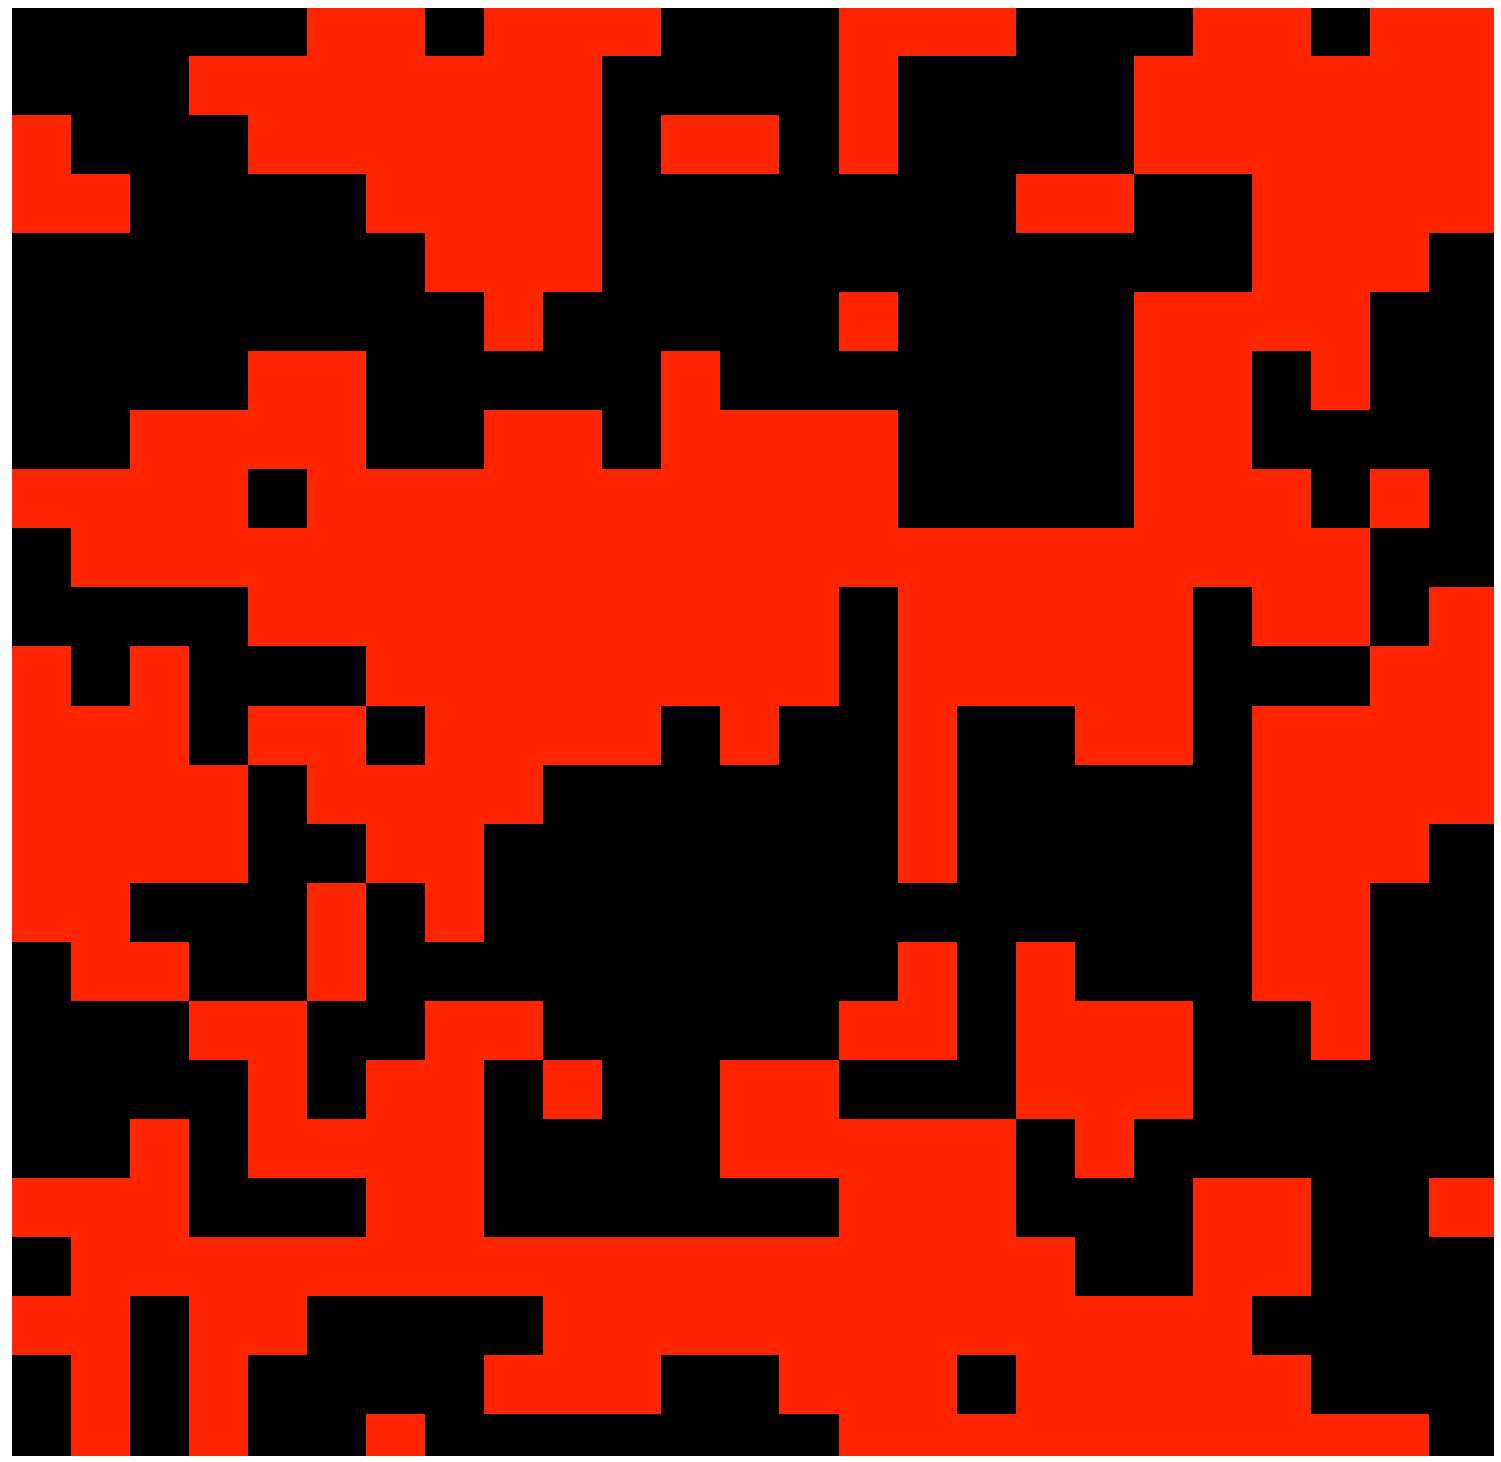
\includegraphics[width=\textwidth]{images/task1/regular_net_Str_t=5000.png} 
    \caption{\scriptsize A-S model, \(t=5000\)}
    \label{reg_net_Str2}
\end{minipage}
\end{figure}







\newpage
\section{Small-world Network}
We study the dynamics on a two-dimensional small-world network to analyze the effect of long-range social interaction. We set \(p = 0.1\).

In agreement with \cite{Castello2008}, we find that long-range interactions inhibit the formation and growth of domains, allowing for long-lived metastable states. However, the system will eventually settle into a dominance-extinction state. 
On the other hand, bilingual agents tend to destroy metastable states of dynamical coexistence and accelerate the decay toward the extinction of one of the languages, as noted by \cite{Castell__2006}.

%due to finite size fluctuactions
%(even if their presence slows down coarsening)

%figures



\begin{figure}[h]
\centering
\begin{minipage}[t]{0.4\linewidth}
    \centering
    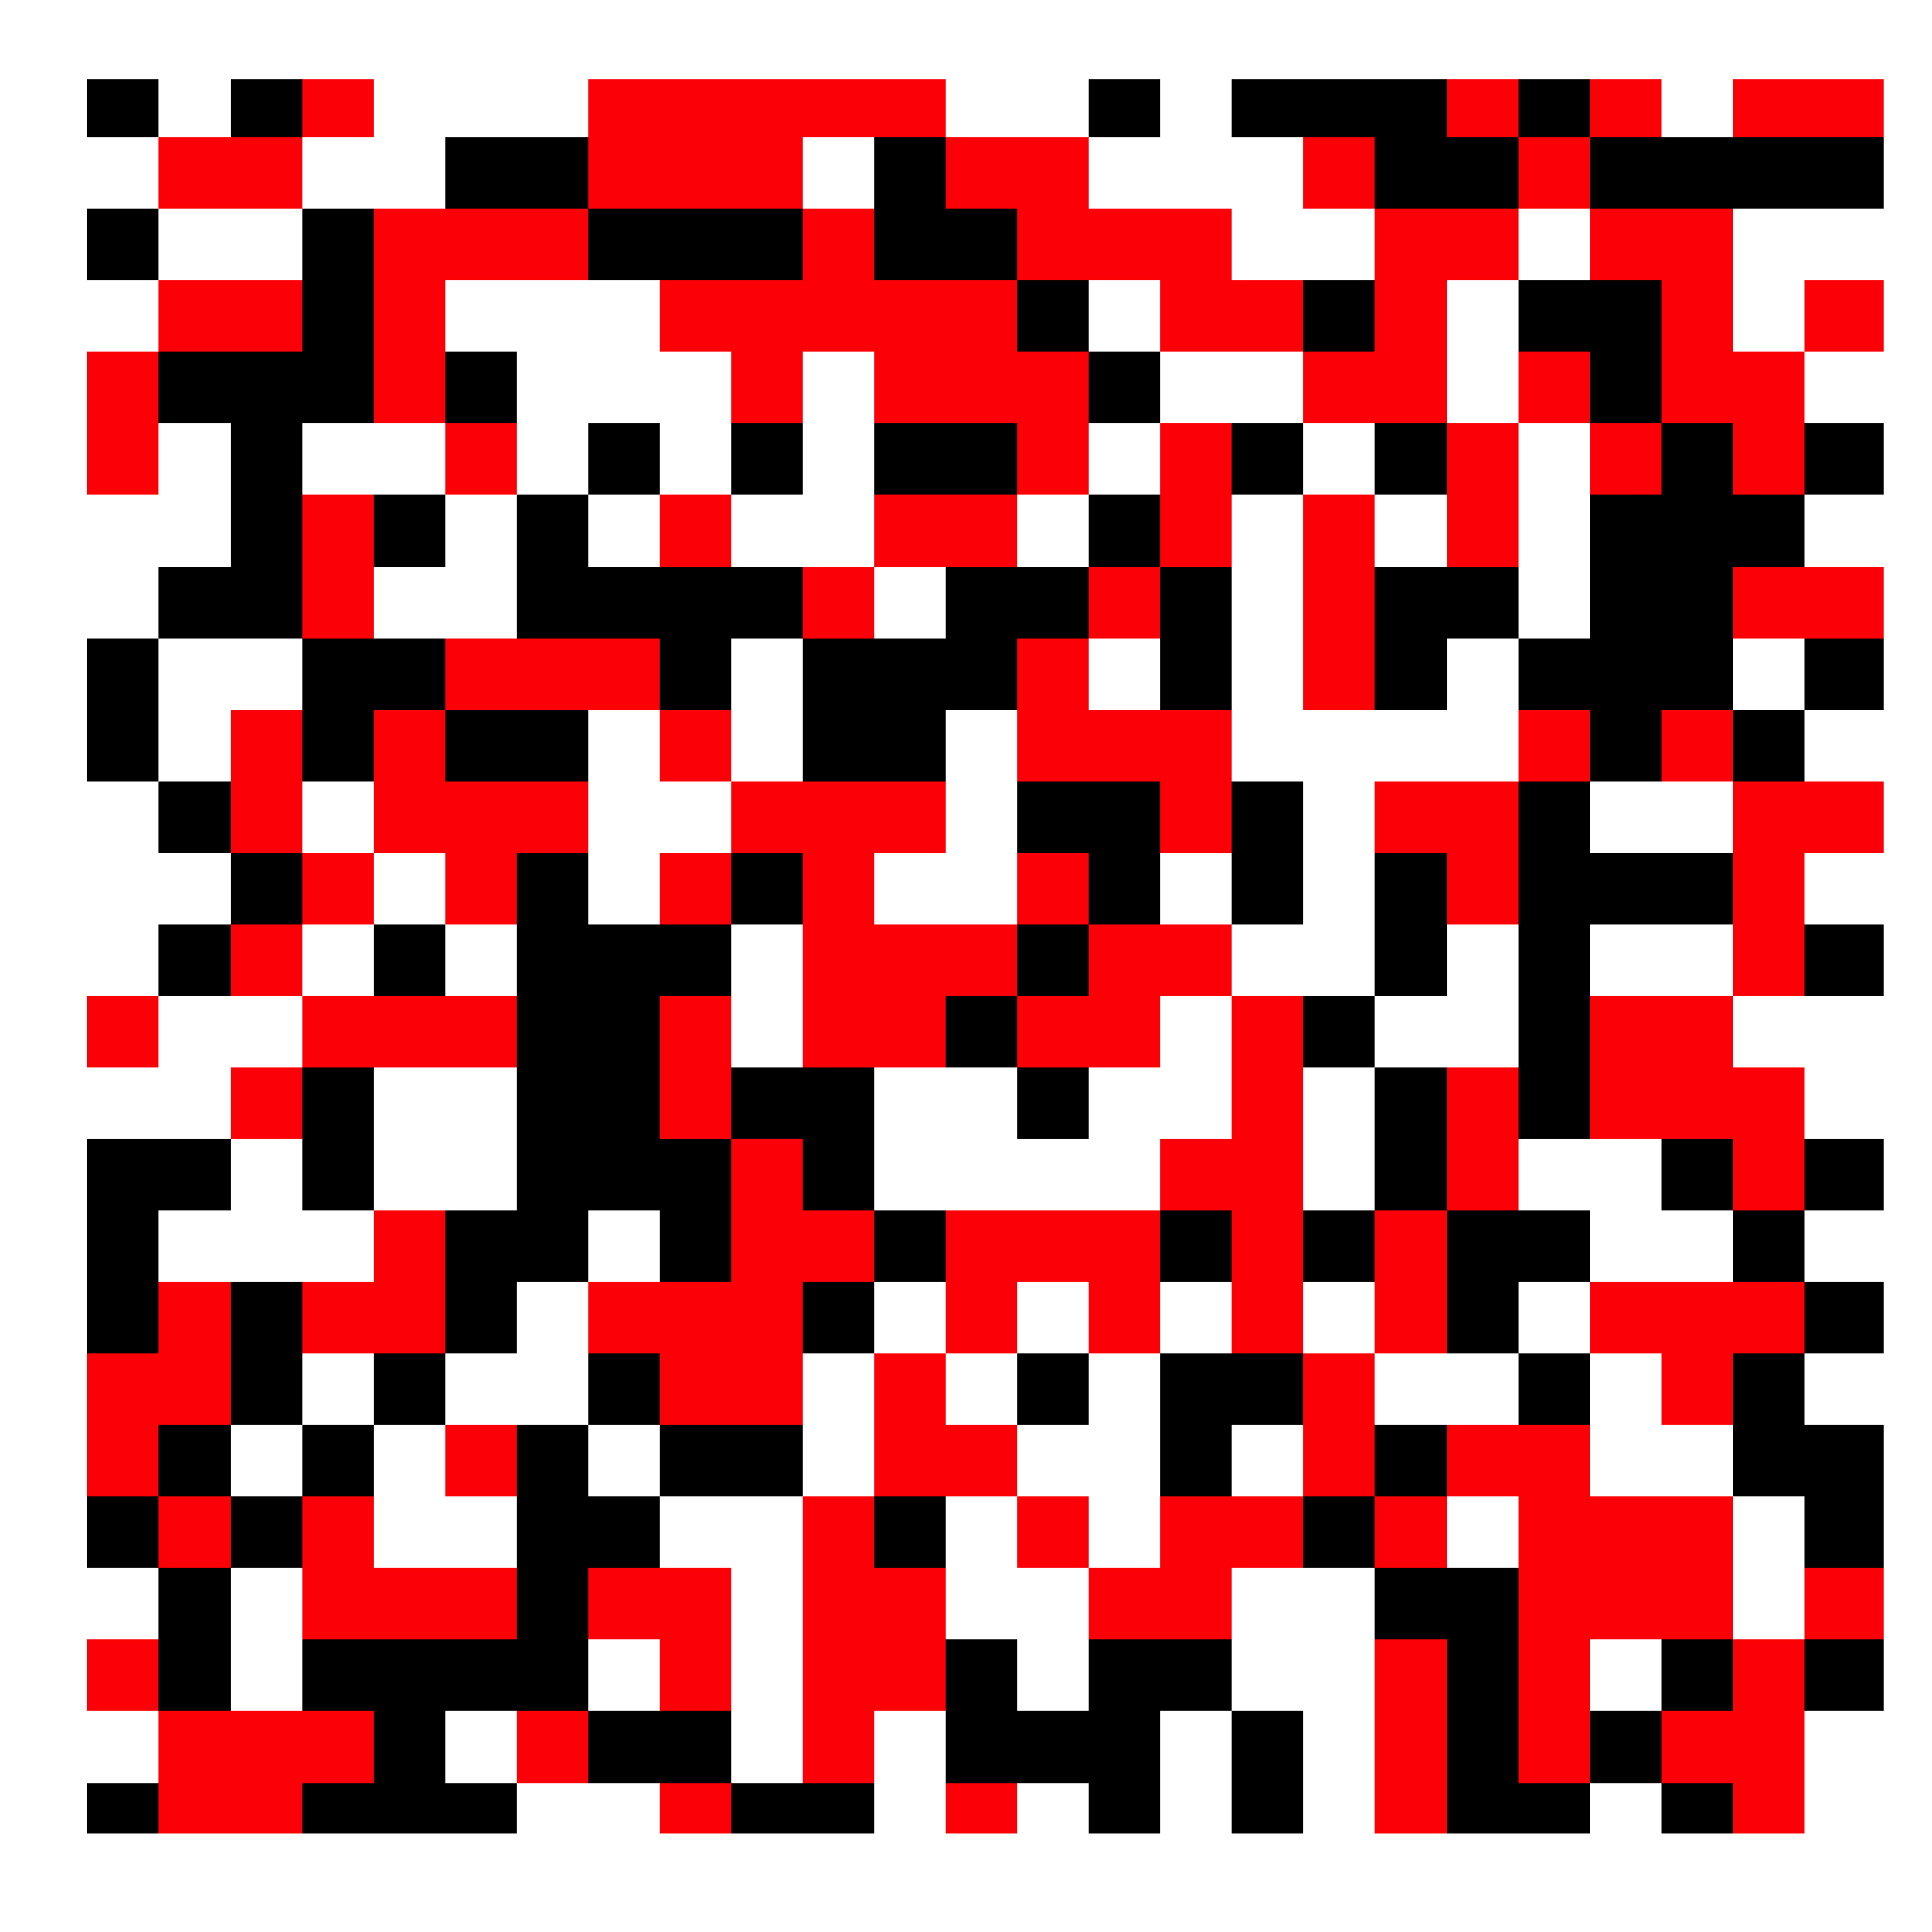
\includegraphics[width=\textwidth]{images/task1/smallw_bi_t=1.png} 
    \caption{\scriptsize Bilingual, \(N=625\), \(t=0\)}
    \label{reg_net_bi1}
\end{minipage}
\hfill
\begin{minipage}[t]{0.4\linewidth}
    \centering
    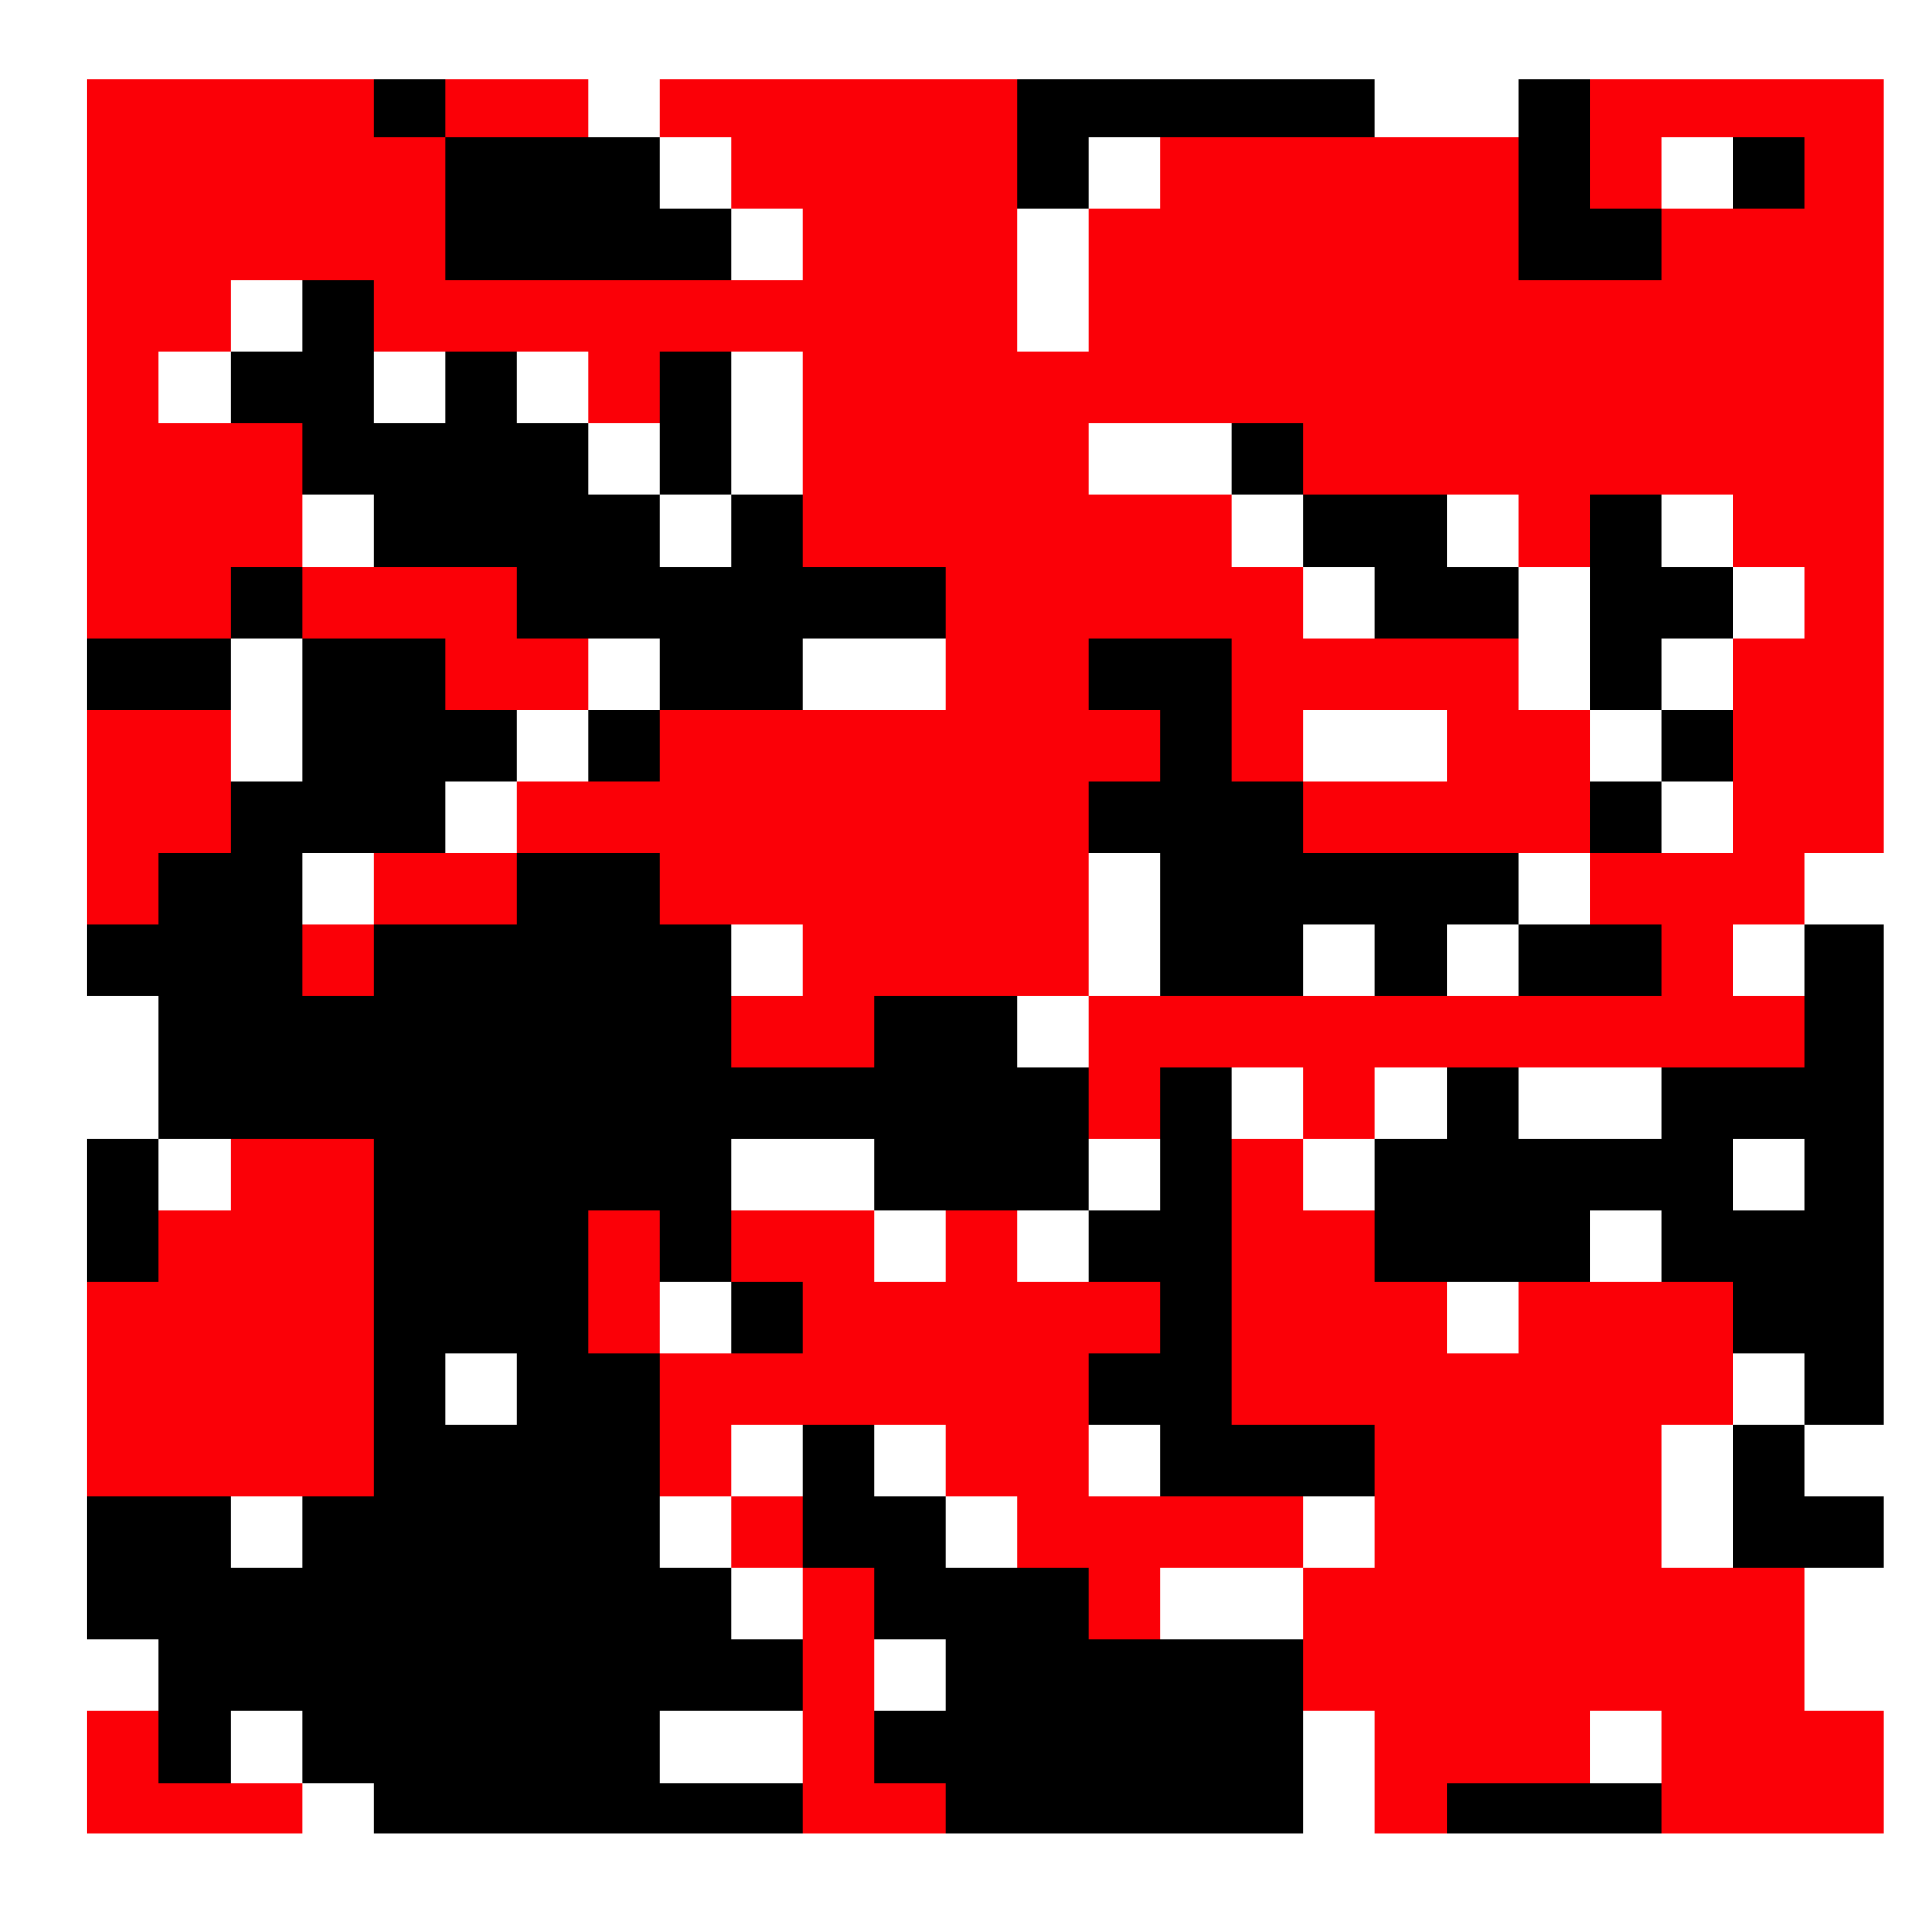
\includegraphics[width=\textwidth]{images/task1/smallw_bi_t=5000.png} 
    \caption{\scriptsize Bilingual, \(t=5000\)}
    \label{reg_net_bi2}
\end{minipage}
\vspace{-5pt}
\begin{minipage}[t]{0.4\linewidth}
    \centering
    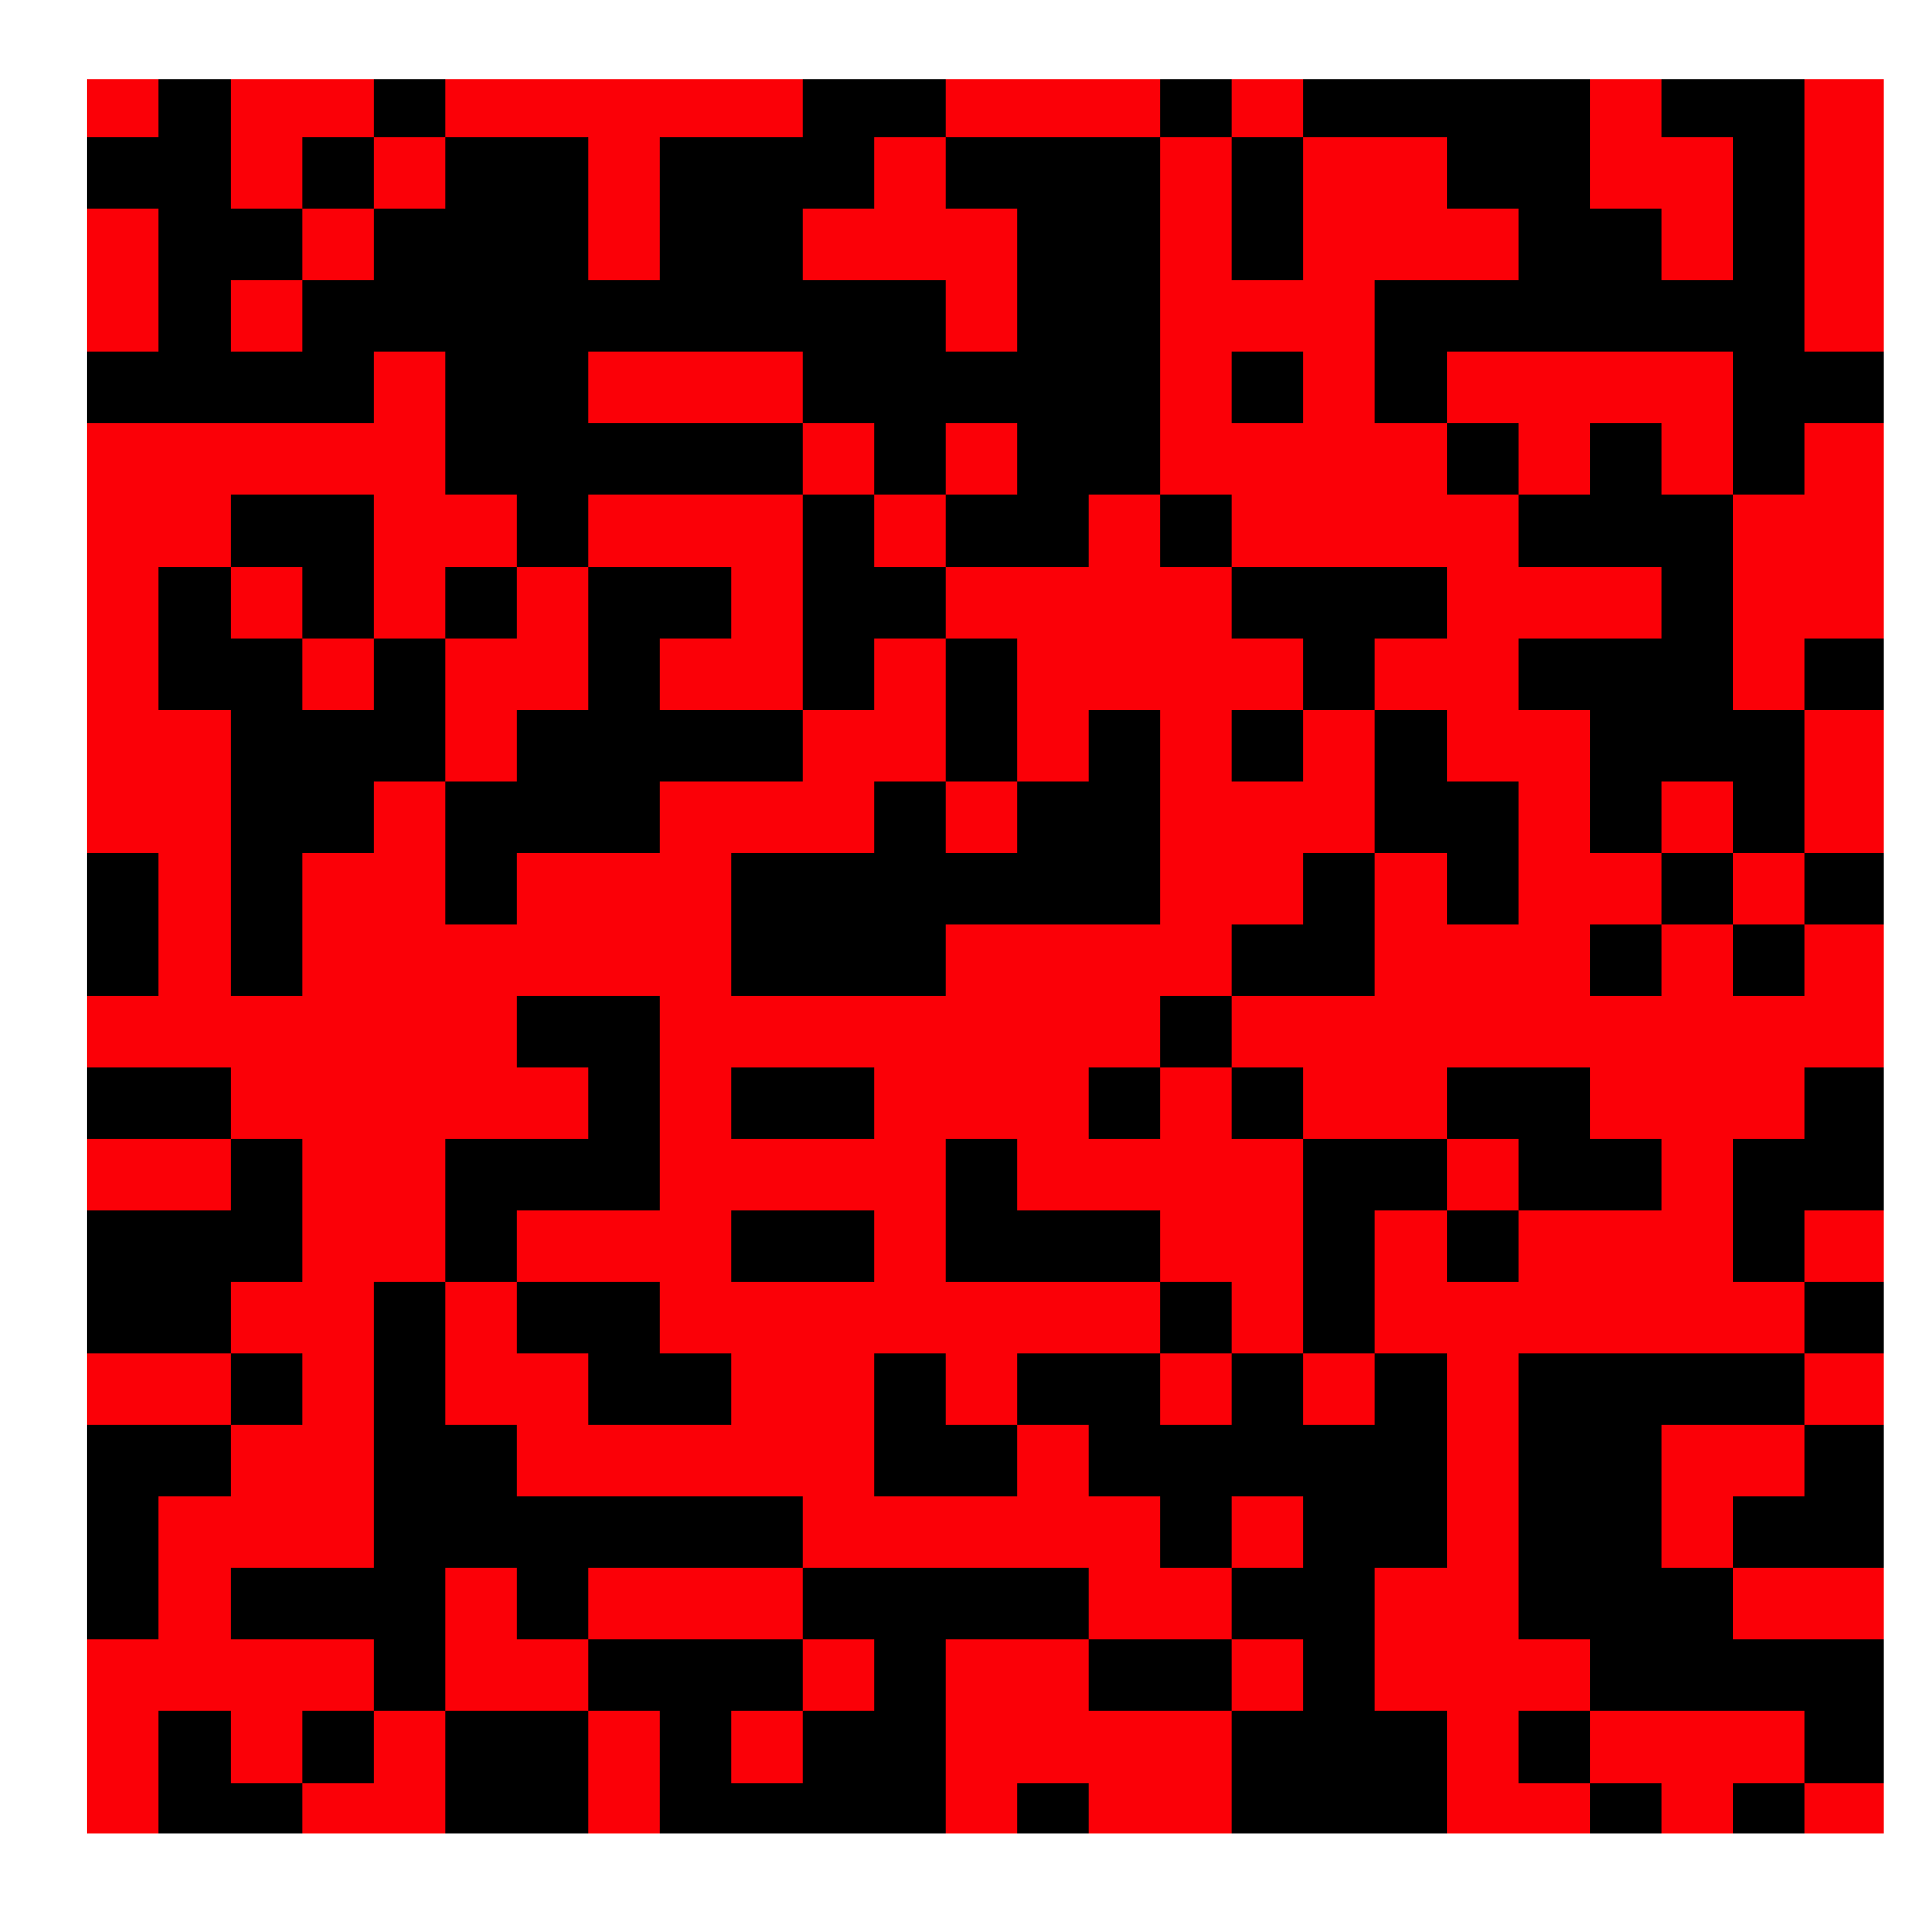
\includegraphics[width=\textwidth]{images/task1/smallw_Strogatz_t=1.png} 
    \caption{\scriptsize A-S model, \(N=625\), \(t=0\)}
    \label{reg_net_Str1}
\end{minipage}
\hfill
\begin{minipage}[t]{0.4\linewidth}
    \centering
    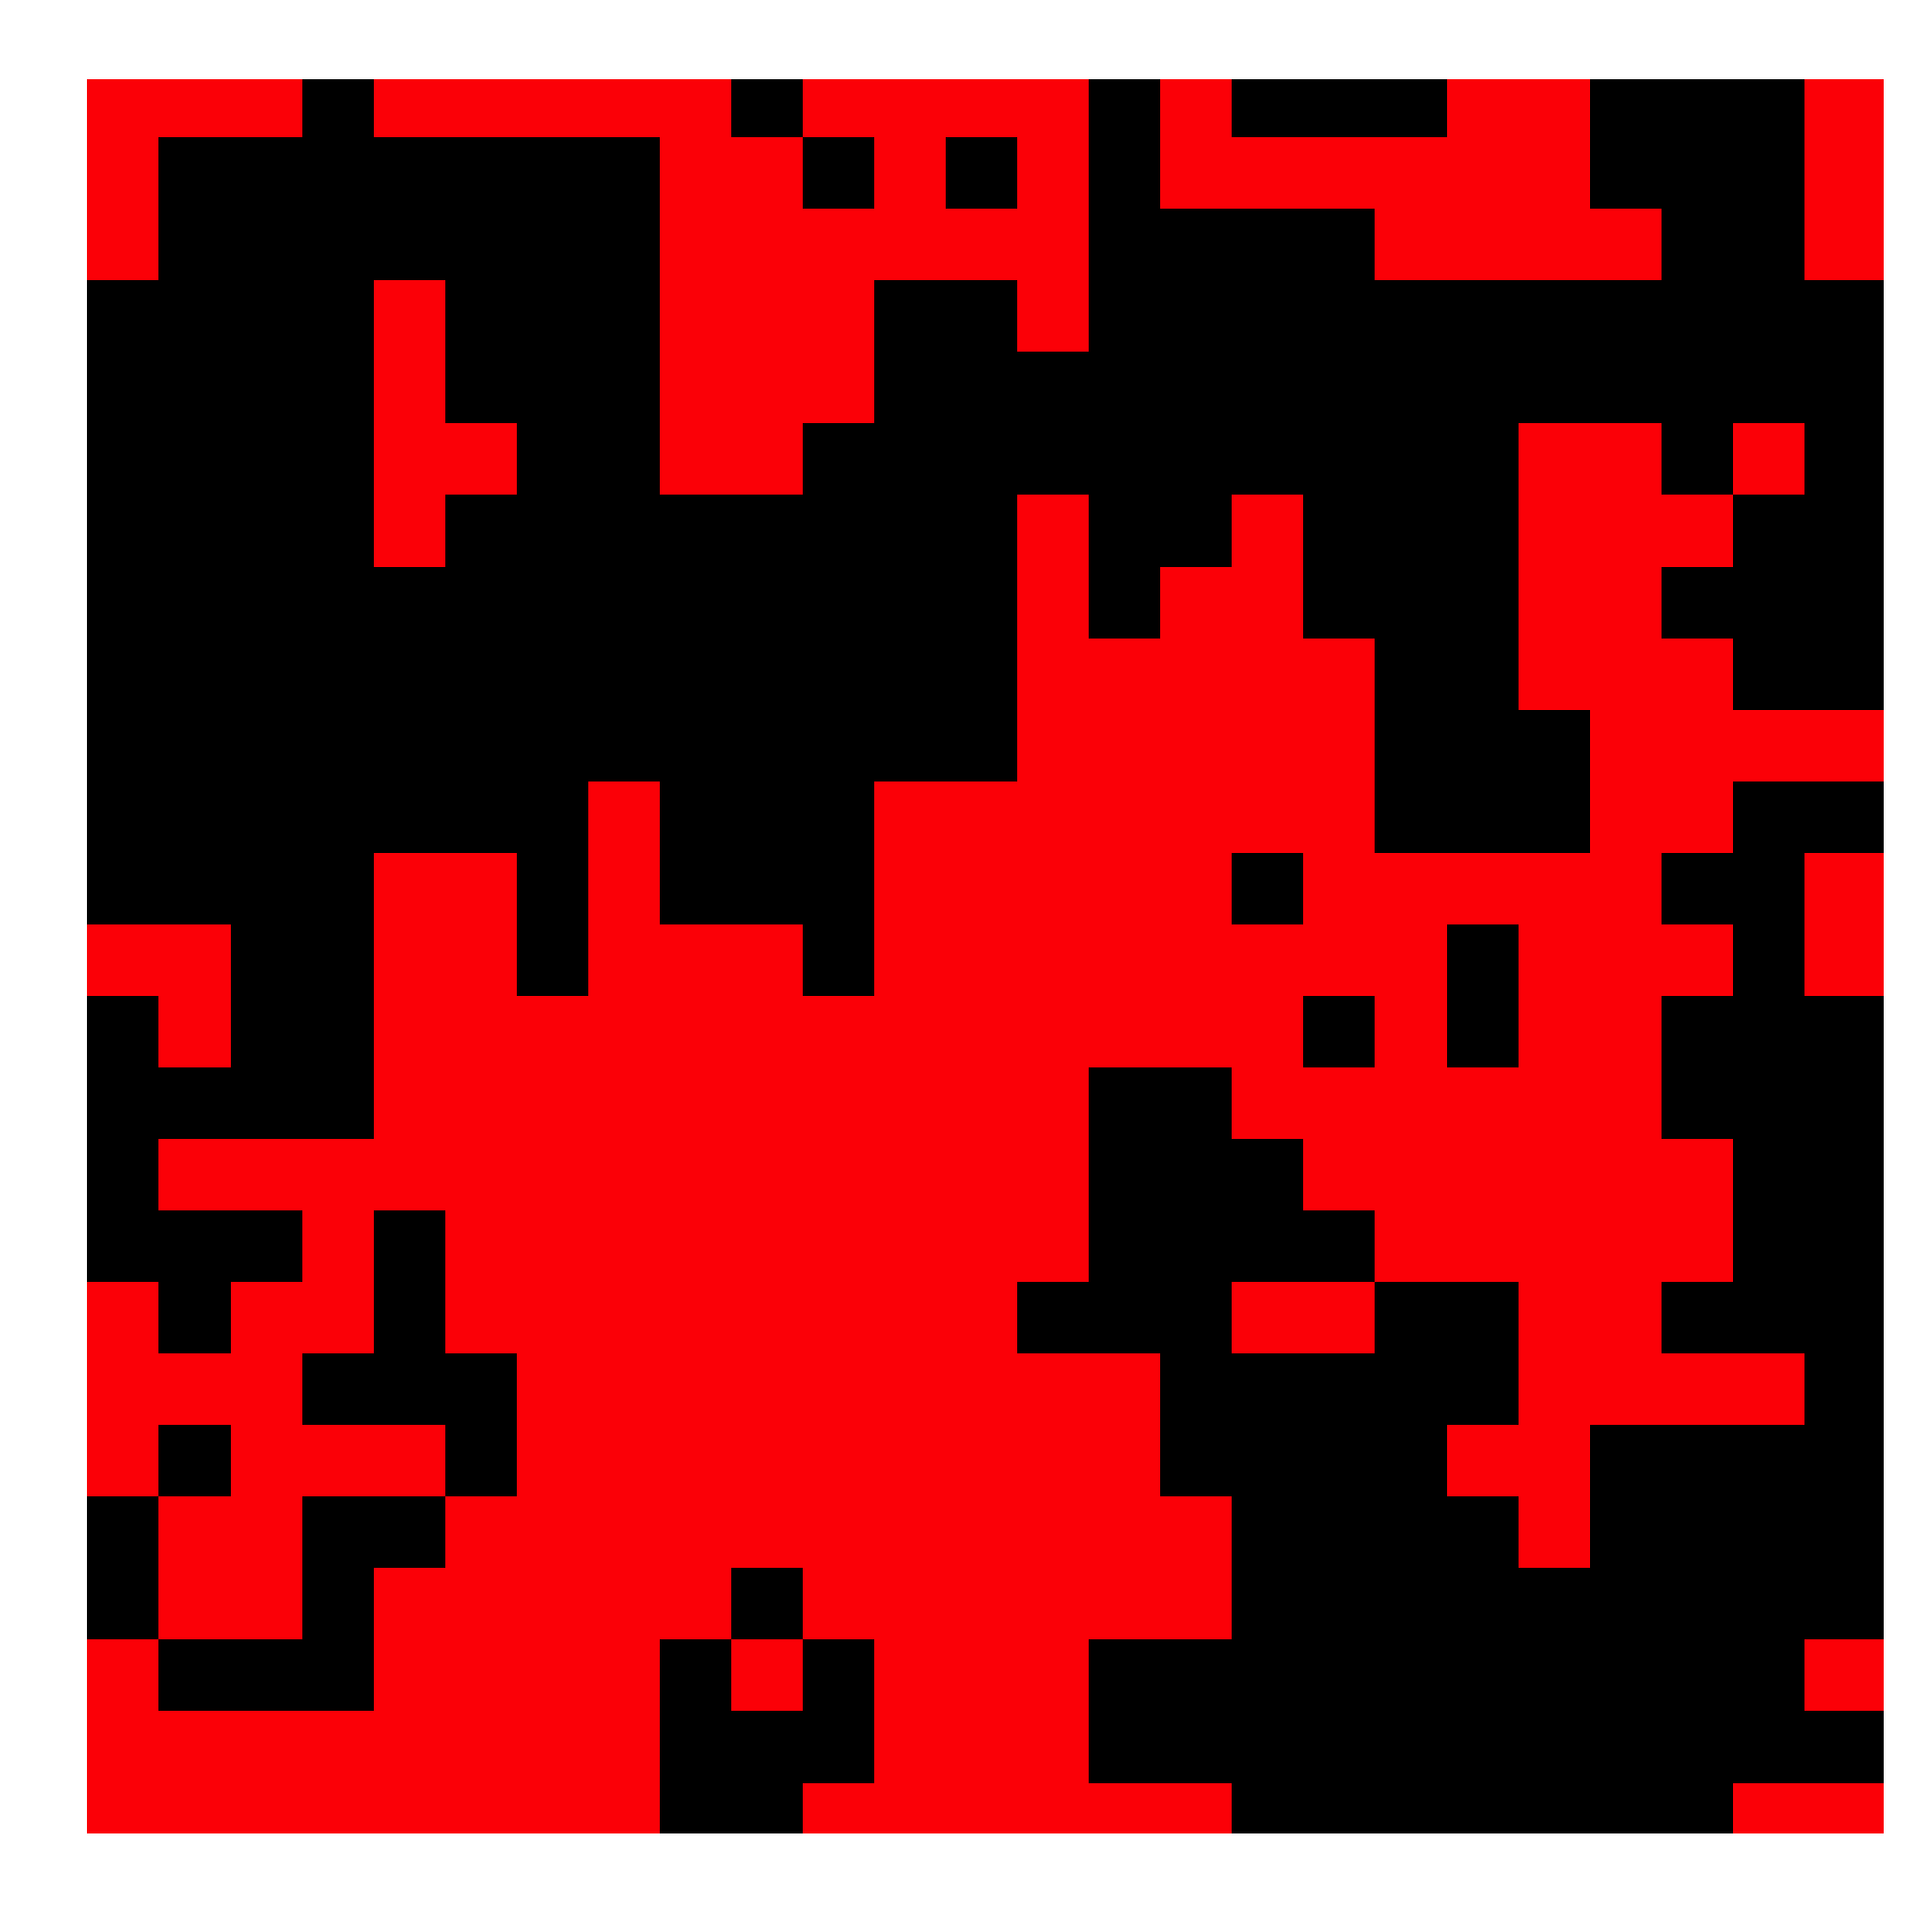
\includegraphics[width=\textwidth]{images/task1/smallw_Strogatz_t=5000.png} 
    \caption{\scriptsize A-S model, \(t=5000\)}
    \label{reg_net_Str2}
\end{minipage}
\end{figure}


In conclusion AB-agents produce an essential modification of the processes of coarsening and domain growth, changing the interfacial noise dynamics of the agent based Strogatz model into a curvature driven interface dynamics.

%###
However, in the topology considered, we haven't been able to reproduce stable bilingual coexistance. In fact it seems that bilingualism is not an efficient mechanism to stabilize language diversity when a social structure of interactions such as the small world network is taken into account. In contrast, bilingual agents are generally found to ease the approach, absorbing monolingual states by an obvious effect of smoothing the communication across linguistic borders.

\chapter*{Remarks}
Part of the code was generated with the assistance of ChatGPT (v4), though never used blindly. For example, it helped build functions for network plotting. Additionally, this tool was helpful in checking grammar and making minor adjustments to improve the readability of this text.

